\documentclass{beamer}

%%% -------------- CREATE HANDOUTS -----------------------------------
%\documentclass[12pt, handout]{beamer}
%\usepackage{pgfpages}
%\pgfpagesuselayout{4 on 1}[letterpaper, landscape, border shrink=1mm]
%%% ------------------------------------------------------------------

\usepackage{ragged2e}
\usepackage[english]{babel}
\usepackage[utf8]{inputenc}
\usepackage{appendixnumberbeamer}
\usepackage{natbib}
\usepackage{textpos}
\usepackage{lipsum}
\usepackage{tikz}
\usepackage[percent]{overpic}
\usepackage{textcomp}
\usepackage{booktabs}
\usepackage{mathabx}
\usepackage{pifont}
\usepackage{bbding}
\usepackage{fontenc}
\usepackage{mathtools}
\usepackage{bm}




\mode<presentation>
  \usepackage{ru}
  %\usetheme{Warsaw}
  %\usecolortheme{seahorse}
  %\usefonttheme{default}
  \setbeamertemplate{caption}[numbered]
  %\setbeamertemplate{headline}{}
  %\setbeamertemplate{navigation symbols}{}
  \setbeamertemplate{bibliography item}[text]
\newcommand*\oldmacro{}%
	\let\oldmacro\insertshorttitle%
%\renewcommand*\insertshorttitle{%
%   \oldmacro\hfill%
%   \insertframenumber\,/\,\inserttotalframenumber}
\setbeamertemplate{section page}{
    \begin{centering}
    \vspace{1cm}
    \begin{beamercolorbox}[rounded=true,shadow=false,sep=4pt,center]{part title}
    \usebeamerfont{section title}\LARGE{\insertsection}\par
    \end{beamercolorbox}
\end{centering}}

%Modify Title page
\title[Decontamination Factors for Nuclear Forensics]{Experimental Characterization of Pu Separation by PUREX Process on a Low-Burnup, Pseudo-Fast-Neutron Irradiated DUO\tsbs{2} for Product Decontamination Factors and Nuclear Forensics}
\institute{Ph.D. Preliminary Examination}
\author{Paul Mendoza}
\date{02/27/2017}

\setbeamertemplate{title page}{
  \begin{centering}
    \vspace{-0.7cm}
    \begin{beamercolorbox}[rounded=true,shadow=false,sep=4pt,center]{part title}
      \usebeamerfont{title}\normalsize{\inserttitle}\par
    \end{beamercolorbox}
    \vspace{0.6cm}
    \begin{tabular}{rl}
    A PhD. Prelims Defense by:      & Paul Mendoza \\[1ex]
    Chair: & Dr. Sunil Chirayath\\[1ex]
    Committee Members: & Dr. Sean McDeavitt\\
    & Dr. Craig Marianno\\
    & Dr. Cody Folden III.
    \end{tabular}
    \begin{center}
      Monday, February 27, 2017, 10:00 am\\
      AIEN 304
    \end{center}
  \end{centering}
}

%Without headline environment
\makeatletter
\newenvironment{withoutheadline}{
  \setbeamertemplate{headline}[default]
  \def\beamer@entrycode{\vspace*{-\headheight}}
}{}
\makeatother

\usebackgroundtemplate{}

%\let\Sun\undefined   %to undefine something
%\usepackage{marvosym}
%\usepackage{scalerel}
%% \usepackage[
%%   style=numeric,
%%   citestyle=authoryeartitle
%% ]{biblatex}
\setbeamerfont{caption}{size=\tiny}

%\setbeameroption{show notes}
%\setbeamertemplate{note page}[plain]
\newcommand{\tss}{\textsuperscript}
\newcommand{\tsbs}{\textsubscript}


%\usepackage{enumitem,amssymb}  %enumitem messes with beamers list settings
%\newlist{todolist}{itemize}{2}
%\setlist[todolist]{label=$\square$}
\usepackage{pifont}
\newcommand{\cmark}{\ding{51}}%
\newcommand{\xmark}{\ding{55}}%
\newcommand{\done}{\rlap{$\square$}{\raisebox{2pt}{\large\hspace{1pt}\cmark}}%
  \hspace{-2.5pt}}
\newcommand{\notdone}{$\square$}
\newcommand{\wontfix}{\rlap{$\square$}{\large\hspace{1pt}\xmark}}

%Change Bullets in latex list
\setbeamertemplate{itemize item}{\scriptsize\raise1.25pt\hbox{\donotcoloroutermaths\ding{118}}}
\setbeamertemplate{itemize subitem}{\scriptsize\raise1.25pt\hbox{\ding{226}}}
\setbeamertemplate{itemize subsubitem}{\tiny\raise1.25pt\hbox{\ding{169}}}
\setbeamertemplate{enumerate item}{\insertenumlabel.}




%%TO SELECT SPECIFIC FONT
%{\FONTSIZE{2.5}{4}\SELECTFONT TOBESIZE}

%BIOLA SEAL
%\SETBEAMERTEMPLATE{BACKGROUND}{\TIKZ[OVERLAY, REMEMBER PICTURE]\NODE[XSHIFT=-2.3CM, YSHIFT=1.50CM, OPACITY=0.4]AT (CURRENT PAGE.SOUTH EAST){\INCLUDEGRAPHICS[WIDTH=4CM]{IMAGES}};}

\begin{document}

%Uncomment for handouts
%\setbeamertemplate{headline}{}

\setbeamertemplate{caption}{\raggedright\insertcaption\par}
\begin{frame}
	%% background
  \tikz[overlay, remember picture]\node[xshift=-3.5cm, yshift=3cm, opacity=0.1]at (current page.south east){
\includegraphics[width=8cm]{figures/tamu_system_proposed_seal_042915}};
	%% Left-hand logo
  \begin{tikzpicture}[remember picture, overlay]
  \node [xshift = 3 cm, yshift=1.2cm] at (current page.south west){
\includegraphics[width=5cm]{figures/tees_logo_primary_maroon}};
  \end{tikzpicture}
    %% Right-hand logo
  \begin{tikzpicture}[remember picture, overlay]
  \node [xshift = -3cm, yshift=1.2cm] at (current page.south east){
\includegraphics[width=5cm]{figures/TEES_NSSPI_logo_HMaroon}};
  \end{tikzpicture}
  
  %% Upper logo right (comment for handouts)
    \begin{tikzpicture}[remember picture,overlay]
    \node[anchor=north east,yshift=2pt] at (current page.north east) {
\includegraphics[height=0.8cm]{figures/NUENlogo}};
    \end{tikzpicture}
  
  %% Upper logo left
    %% \begin{tikzpicture}[remember picture,overlay]
    %% \node[anchor=north west,yshift=2pt] at (current page.north west) {
\includegraphics[height=0.8cm]{NUENlogo}};
    %% \end{tikzpicture}

    \titlepage
    %\vspace{-1.8cm}
    %\begin{center}
    %  Presented at All Hands Meeting
    %\end{center}
\end{frame}

%Add Biola Seal
\setbeamertemplate{background}{\tikz[overlay, remember picture]\node[xshift=-2.5cm, yshift=2.5cm, opacity=0.05]at (current page.south east){
\includegraphics[width=6cm]{figures/imageedit_2_7317234434}};}

%Add NSSPI to upper right (comment for handouts)
\addtobeamertemplate{frametitle}{}{%
  \begin{tikzpicture}[remember picture,overlay]
    \node[anchor=north east,yshift=2pt] at (current page.north east) {
\includegraphics[height=0.8cm]{figures/NUENlogo}};
  \end{tikzpicture}
    \begin{tikzpicture}[remember picture,overlay]
      \node[anchor=north west,yshift=2pt] at (current page.north west) {
\includegraphics[height=0.8cm]{figures/TEES_NSSPI_Acronym_logo_WHT}};
  \end{tikzpicture}
}


\begin{frame}{Outline}
\tableofcontents
\end{frame}

\section{Introduction}

\subsection{Motivation}
\begin{frame}{Motivation}
  \begin{itemize}
  \item{Current Events}
    \begin{itemize}
    \item{Joint Comprehensive Plan of Action}
    \item{Non-safeguarded reactors}
    \item{Islamic State of Iraq and Syria}
    \end{itemize}
  \item{Past Events}
    \begin{itemize}
    \item{Septemer 11, 2001}
    \end{itemize}
  \item{Limited scope of IAEA safeguards}
  \item{``the awful arithmetic of the atomic bomb''\tss{\cite{RN212}}}
  \item{Need for improved forensic capabilities\tss{\cite{RN103,RN98,RN113}}}
  \end{itemize}
\end{frame}

\note{Wanted to take some time to talk about the motivation behind this project.
  There are a lot of stuff going on in the world. Here I've listed a few that pertain to nuclear
  weapons.
  \begin{itemize}
  \item{Iran limiting capabilities for 8 years}
  \item{non-safeguarded reactors, in India for example}
  \item{North Korea, detonating a nuclear device October 2006}
  \item{ISIS, if they could, would probably want nuclear weapons, and they would use them on us}
  \end{itemize}
  As 911 indicated, we have enemies, who don't like us. To quote William Perry,
  ``Our greatest threat is a terrorist nuclear strike''. Lukily, aquiring nuclear weapons
  is no easy task. And thanks to organizations like the international atomic energy agency,
  or the treaty on the non proliferation of nuclear weapons, the international community is
  generally on board with nonproliferation. Nontheless, all sources of special nuclear material
  are not safeguarded, and the ``awful arithmetic of the atomic bomb'', to quote Eisenhower,
  doesn't leave much room for calculational errors.
  \begin{itemize}
  \item{Forensic capabilities need to improve, which we will talk about in a minute,
  but first, some definitions}
  \end{itemize}
}

\begin{frame}{Definitions}
  \vspace{-0.7cm}
  \begin{itemize}
  \item{Special Nuclear Material (SNM)}
    \begin{itemize}
    \item{Plutonium, \tss{233}U, or \tss{235}U}
    \end{itemize}
  \item{Nuclear Forensics}
    \begin{itemize}
    \item{The investiative activity that surrounds the search for attributes
      of undetermined radioactive specimens for the purpose of attribution.}
    \end{itemize}
  \item{SNM origin attributes/indicators}
    \begin{itemize}
    \item{Indicators or clues for SNM origin attribution. Examples include burnup, fluence rate,
    initial fuel enrichment, fuel age, and fast-to-thermal irradiation ratios}
    \end{itemize}
  \item{Decontamination Factors (DF)}
    \begin{itemize}
    \item{A measure of the effectiveness with which a product is decontaminated from a
      contaminant}
    \end{itemize}
  \end{itemize}
  \vspace{1mm}
    \begin{equation*}
      DF_j=\frac{\frac{c_j}{c_{Pu}}|_{\text{initial}}}{\frac{c_j}{c_{Pu}}|_{\text{final}}}
    \end{equation*}
\end{frame}

\note{At this point I wanted to take a moment to define some terms. To help narrow our
  nonproliferation scope. First,
  \begin{itemize}
  \item{Special nuclear material, this is the material that is traditionally safeguarded. One of
    three building blocks for nuclear weapons, which are the material, design information,
    and manufacturing skills}
  \item{Nuclear forensics - investigative activity, determing attributes of SNM. This could
    include composition, material form, or date since processing. Involves a broad range of
    scientific destructive and nondestructive techniques. The time scale for full nuclear
    forensic analysis for samples can vary widely, depending on the prepardness of whatever
    laboratory is receiving the sample. In Moody's book, nuclear forensic analysis, he cites
    several examples that took a couple of months to analyze}
  \item{For my project I will be determining several attributes or indicators for a sample.
    I wanted to note that these indicators are clues or evidence towards a conclusion. And the
    examples listed are indicators that I would like to determine.}
  \end{itemize}
}


\subsection{Contexts}
\begin{frame}{National Context}
  \vspace{-1cm}
  \begin{center}
    ``The United States has developed a nuclear forensics capability that has been demonstrated
    in real-world incidents of \textbf{interdicted materials} and in exercises of actions
    required after a nuclear detonation. The committee, however, has concerns about the program
    and finds that without strong leadership, careful planning, and additional funds, these
    capabilities will decline''\tss{\cite{RN103}}
  \end{center}
  Major areas of concern include:
  \begin{itemize}
  \item{Organization}
  \item{Sustainability}
  \item{\textbf{Workforce and Infrastructure}}
  \item{\textbf{Procedures and Tools}}
  \end{itemize}
\end{frame}

\note{According to a report from the committee on nuclear forensics released in 2010,
    the United States forensic capability has been demonstrated in real world scenarios, but
    is at risk unless certain developmental requirements are met. The committee listed 4 areas
    of concern, where improvment is needed.
    \begin{itemize}
    \item{In terms of organization, nuclear forensics responsibility is shared by several agencies
      without central authority and with no consensus on strateic requirements to guide the program.}
    \item{For sustainability, our current capabilities are the fruit of the nuclear weapons program
      and our laboratory infrastructure, funding for both have been decling}
    \item{Skilled personnel in these areas are few, and key facilities are in need of replacement
      because they are old, outdated, or do not met modern environmental, health, or safety standards.}
    \item{In recent years, nuclear forensic techniques methodologies have been on the rise, some
      from presented from our own department, but according to this source, a large fraction
      of techniques are remnants of the cold war era, with less restrictions. Also, forensic
      excersises usually take months to complete, a time scale which is too long}
\end{itemize}}
\newpage
\note{Problem must be met on an administrative level, but this project will help with two of these
  important goals. Developing the workforce, by example of yours truly, and the procedures we'll talk
  about in a moment.}


\begin{frame}{Forensic Context}
  \begin{itemize}
  \item{Nature of inverse problems}
  \item{Plutonium purification necessary for weapons production}
    \begin{align*}
      ^{238}U+n\rightarrow ^{239}U \xrightarrow[T_{1/2}=23\text{ min}]{\beta^-} ^{239}Np
      \xrightarrow[T_{1/2}=2\text{ d}]{\beta^-}^{239}Pu
    \end{align*}
  \item{Attribution for unpurified Pu has been previously studied
    \tss{\cite{chirayath2015trace,scott2005nuclear,glaser2009isotopic}}}
  \end{itemize}
  \begin{figure}[H]
    \vspace{-3mm}
      \begin{center}
        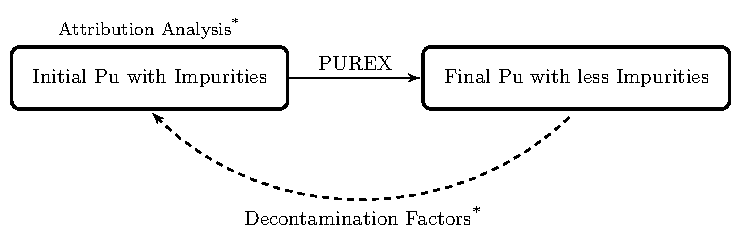
\includegraphics[scale = 0.7]{figures/purpose}
      \end{center}
    \end{figure}
\end{frame}
\note{
  \begin{itemize}
  \item{Inverse problems, naturally have many solutions. Where many paths could be taken to arrive
    at an end state}
  \item{our study will analyze plutonium production, which muddies waters more in its production than
  uranium}
  \item{Purification necessariy because there is a chance for fission along any point of production}
  \item{This complicates attribution by a considerable amount due to unknown DF values}
  \item{Studies have looked at isotopic compositions of irradiated fuel and came to conclusions about
    origins}
  \item{Describe the picture, and how it shows your project, also talk about the assumption...}
  \item{This requires that the specifics of the PUREX process used for plutonium separation are known,
    so that DFs are applied appropriately.}
  \item{If this information were not readily available, this same analysis would have to ensue with
    best estimate PUREX processes and experimentally determined Distribution Coefficients}
  \end{itemize}
}


\begin{frame}{Nuclear Context}
  %\vspace{-1cm}
  \begin{itemize}
  \item{Weapons-grade Pu can be extracted from reactor discharged fuel
    with a burnup of about 1 (GWD/tU)}
  \item{Pu isotopes produced in irradiated fuel can vary} %depending on}
  \item{Two examples of reactors which can intentionally
  discharge low burned fuel for extracting weapon-grade Pu are:}
  \begin{itemize}
  \item{Fast Breeder Reactor, CANDU Reactor}
  \end{itemize}
  \end{itemize}
  \begin{figure}[H]
    \vspace{-3mm}
      \begin{center}
        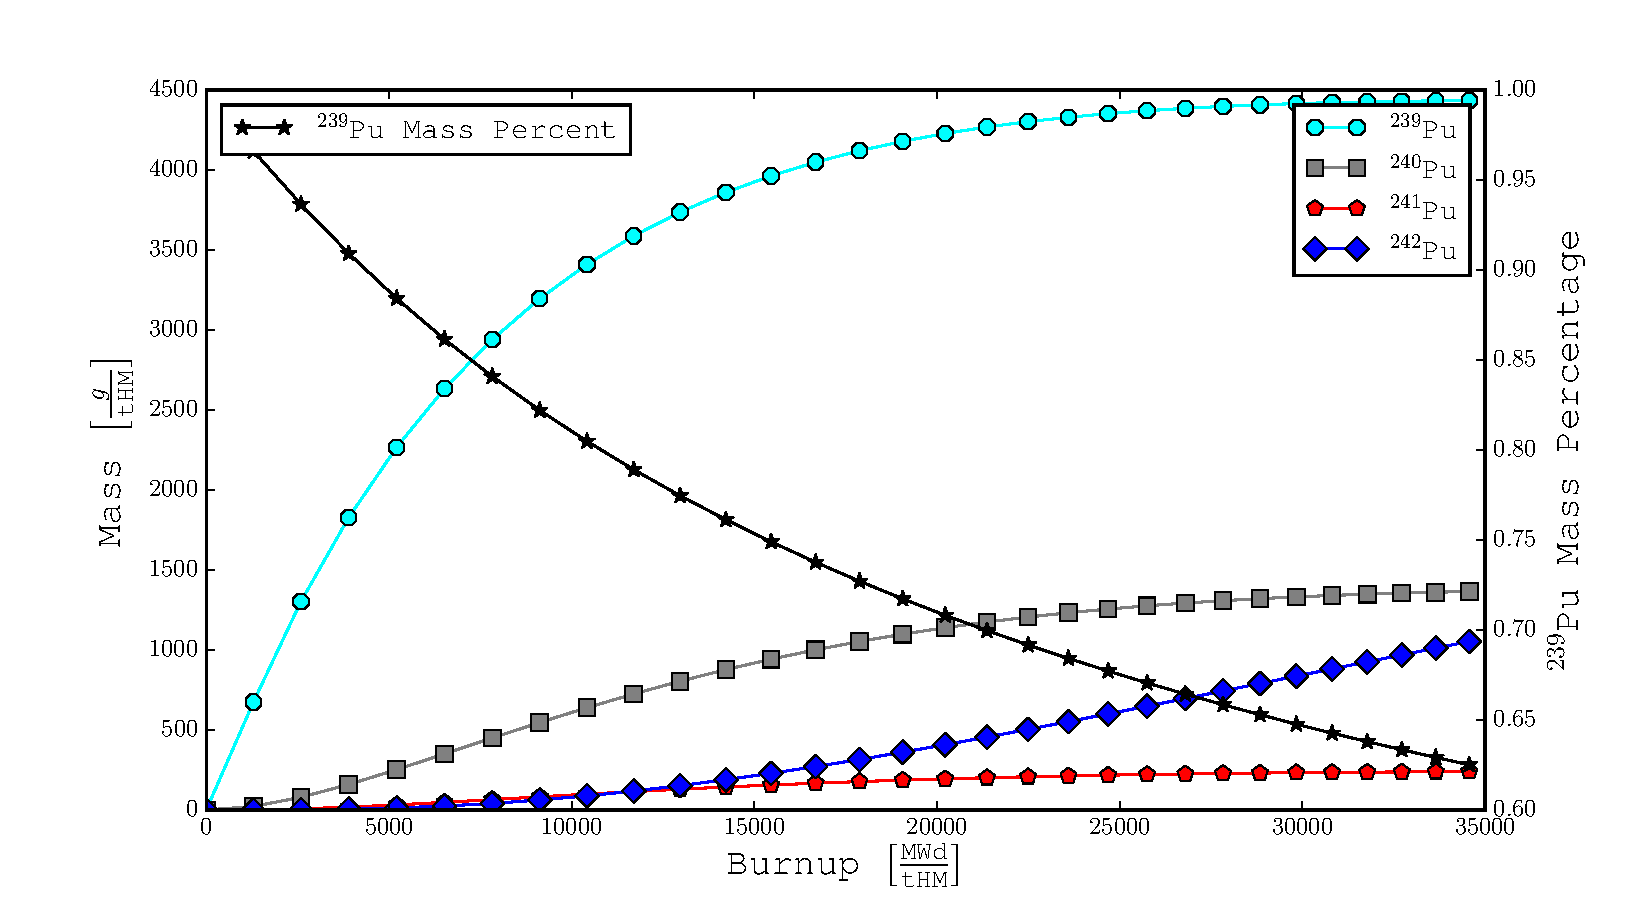
\includegraphics[scale = 0.26]{figures/BurnPuComp_grams}
      \end{center}
    \end{figure}
%\item{In accord with the Indo-US 123 agreement, these reactors were not
%      required to be kept under IAEA safeguards}
  %% \begin{tikzpicture}[remember picture, overlay]
  %%   \node [xshift = -3cm, yshift=1.2cm] at (current page.south east){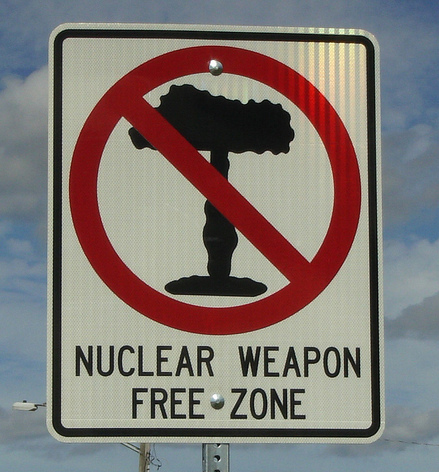
\includegraphics[width=5cm]{nuclear-weapons-free-zone}};
  %% \end{tikzpicture}
\end{frame}
\note{
  \begin{itemize}
  \item{Lower burnup fuel produces weapons}
  \item{Plutonium isotopics depend on }
    \begin{itemize}
    \item{Burnup (irradiation history)}
    \item{Reactor neutron spectrum (core design)}
    \end{itemize}
  \item{Fast Breeder Reactor}
    \begin{itemize}
    \item{Madras Atomic Power Station Kalpakkam, India}
    \item{Expected criticality in Jan 2017}
    \item{Cost from 450 million euros to 750 euros}
    \item{Sodium-cooled reactor design - U238 for breeding}
    \item{100 GWd/t for core, 40 year life, 1750 tonnes of sodium
      about 75\% of olympic sized swimming pool.}
    \item{liquid sodium has a density a little less than water}
    \item{MOX fuel (UO2 and PuO2) fuel}
    \item{Fuel discharged at 100GWd/t, but I just mentioned
      that we are worried about 1GWd/t, mistake?}
    \end{itemize}
  \end{itemize}
}

\begin{frame}{Chemical Context}
  \begin{itemize}
  \item Plutonium Uranium Redox EXtraction (PUREX)
    \begin{itemize}
    \item Liquid-liquid solvent extraction
    \item Many stages:
    \end{itemize}
  \end{itemize}
  \begin{itemize}
  \item{Distribution Coefficient (D): The ratio between the organic
  and aqueous phases (aka: D-values)}
    \begin{equation*}
      D=\frac{c_{o}}{c_{aq}}
    \end{equation*}
    \begin{itemize}
    \item{Specific element to element}
    \item{Vary widely\tss{\cite{stoller1961reactor}}}
    \item{The fraction of mass, $f_o$ deposited in the organic
      phase, assuming a volume ratio between
      the aqueous and organic phases, $V_R$, is:}
    \end{itemize}
    \begin{equation*}
      f_o=(1+D^{-1}V^{-1}_R)^{-1}
    \end{equation*}
  \end{itemize}
\end{frame}

\note{
  \textbf{PUREX Process}
  \begin{enumerate}
  \item{Preparation for Dissolution}
  \item{Dissolution}
  \item{Preparation of Dissolved Feed}
  \item{Primary Decontamination - Extraction to
    organic\textsuperscript{\tiny{\AsteriskThin}}}
  \item{Scrubbing}
  \item{Plutonium Partition - Back-Extraction to
    aqueous\textsuperscript{\tiny{\AsteriskThin}}}
  \item{Plutonium Purification}
  \end{enumerate}
  \textbf{Distribution Coefficients (process depends on this)}
  \begin{enumerate}
  \item{Distribution coefficients can be reported
      in terms of volume basis (weight per unit volume), or a
      mass basis (mass of solute per unit mass of solute free
      solvent)- usually reported on volume basis}
  \item{Vary Widely with: Composition of phases, solution saturation, temperature of the solvent}
  \item{Note: Not a function of desnity, even though the two solutions have different densities,
    when solving for this value, it cancels out}
  \item{Volume matters, Barnwell process has different volumes, more intuitive sense of things}
  \end{enumerate}
}


\begin{frame}{Chemical Context}
  \begin{columns}
    \begin{column}{0.5\textwidth}
      \vspace{-10mm}
      \begin{itemize}
      \item{Lack of literature on decontamination factors and
        distribution coefficients for useful forensic elements (Cs, Sb,
        Eu, Rb, Sr, Nd, Pm, and Sm)}
      \item{With a known process and D-values, DF values for individual elements can
        be determined}
      \end{itemize}
    \end{column}
    \begin{column}{0.5\textwidth}
      \begin{figure}[H]
        \vspace*{-1cm}
        \begin{center}
	  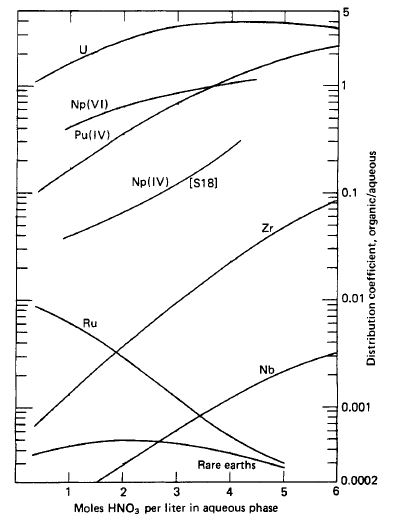
\includegraphics[scale = 0.5]{figures/Stoller}
          \vspace{-0.5cm}
           \caption{\tiny{Adapted from Stoller\tss{\cite{stoller1961reactor}}}}
	\end{center}
      \end{figure}
    \end{column}
  \end{columns}  
\end{frame}


\subsection{Background}



\begin{frame}{Extraction}
  $UO_{2(aq)}^{2+}+2NO^{-}_{3(aq)}+2TBP_{(o)}
  \leftrightarrow UO_2(NO_3)_2\cdot2TBP_{(o)}$\tss{\cite{benedict1982nuclear}}
  $Pu^{4+}_{(aq)}+4NO^{-}_{3(aq)}+2TBP_{(o)}
  \leftrightarrow Pu(NO_3)_4\cdot 2TBP_{(o)}$
  \vspace{-3mm}
  %% \begin{center}
  %% \begin{tikzpicture}
  %%   \node (img1) {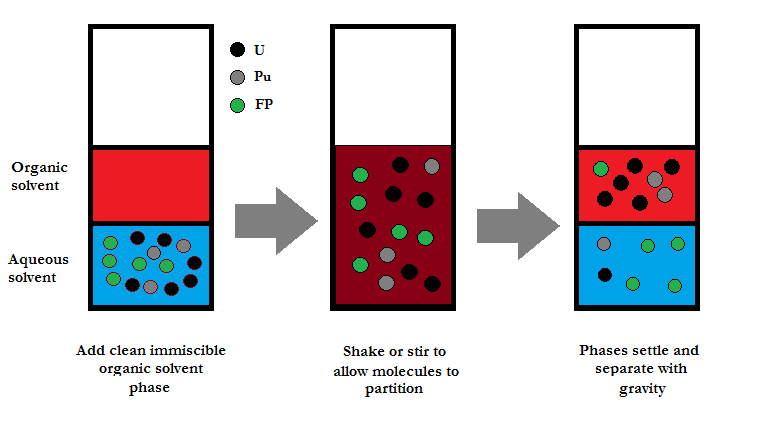
\includegraphics[scale=0.5]{figures/Extraction}};
  %%   \pause
  %%   \node (img2) at (img1.north west) {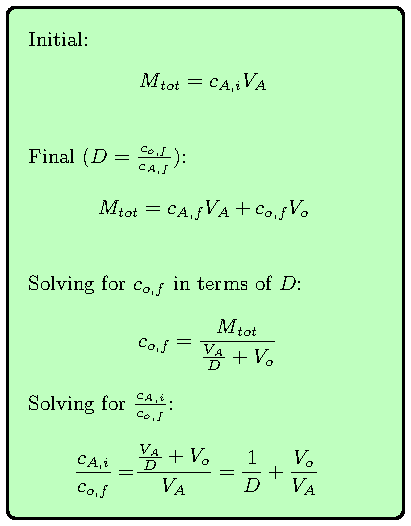
\includegraphics[height=3cm]{figures/Extraction1}};
  %%   \pause
  %%   \node (img3) at (img1.north west) [yshift=1cm] {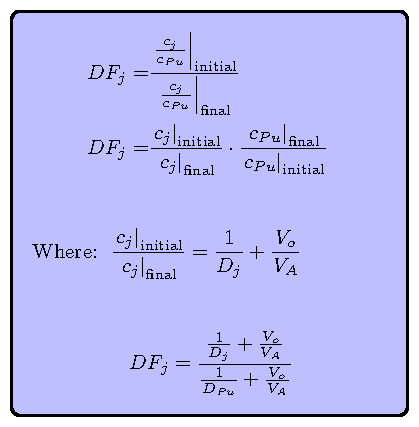
\includegraphics[height=3cm]{figures/Extraction2}};
  %% \end{tikzpicture}
  %% \end{center}
  \begin{figure} \centering
    \vspace*{0.1cm}
    \begin{tikzpicture}[
        every node/.style={anchor=south west,inner sep=0pt},
        x=1mm, y=1mm,
      ]
      \node (fig1) at (0,0)
            {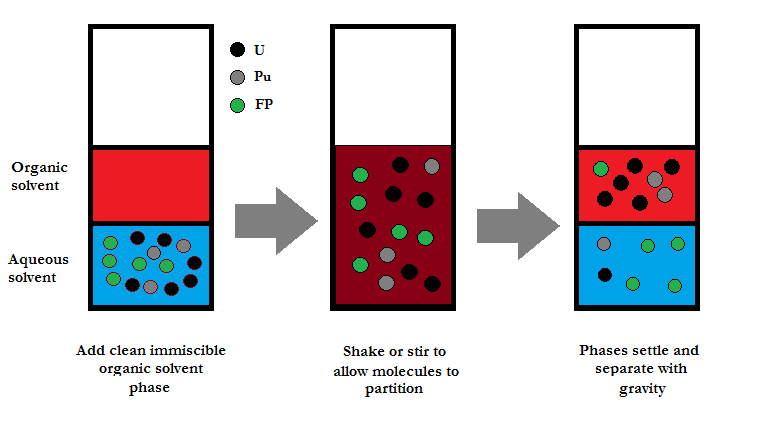
\includegraphics[scale=0.5]{figures/Extraction}};
      \pause
      \node (fig2) at (30,5)
            {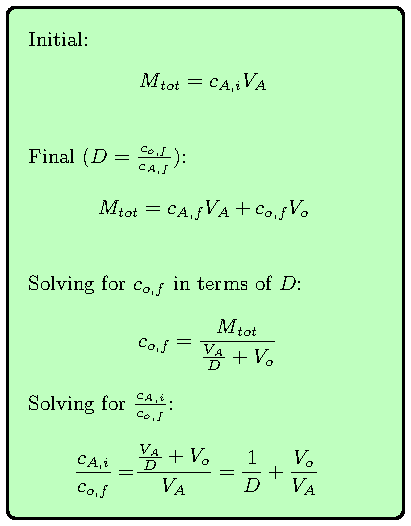
\includegraphics[scale=0.6]{figures/Extraction1}};
      \pause
      \node (fig3) at (30,15)
            {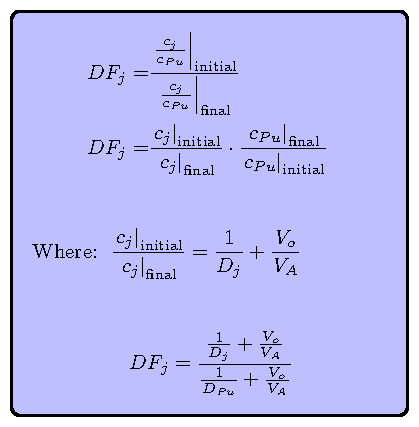
\includegraphics[scale=0.6]{figures/Extraction2}};      
            
    \end{tikzpicture}
    \caption{Using Tikz Overlay}
  \end{figure}
  %% \begin{figure}[H]
  %%   \vspace*{0.1cm}
  %%   \begin{center}
  %%     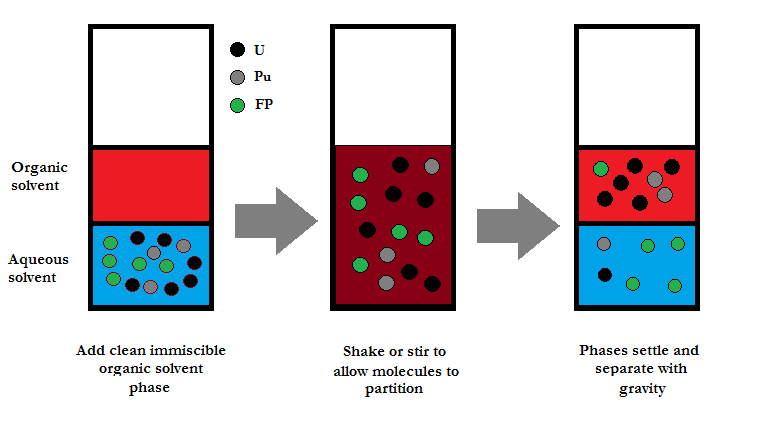
\includegraphics[scale = 0.5]{figures/Extraction}
  %%   \end{center}
  %% \end{figure}
\end{frame}
\note{
  \begin{itemize}
  \item{For the PUREX process, there are two main separation steps, for which
    we will look at more closely}
  \item{Most of the fission products are
    left in the aqueous solution
    at valence III and V states\tss{\cite{kok2009nuclear}}}
  \end{itemize}
}

\begin{frame}{Back-Extraction}
  $Pu(NO_3)_4(TBP)_{2(o)}+Fe^{2+}_{(aq)}\leftrightarrow Pu^{3+}_{(aq)}+4NO^{-}_{3(aq)}+2TBP_{(o)}$\tss{\cite{konings2006chemistry}}
  %% \begin{figure}[H]
  %%   \vspace*{0.1cm}
  %%   \begin{center}
  %%     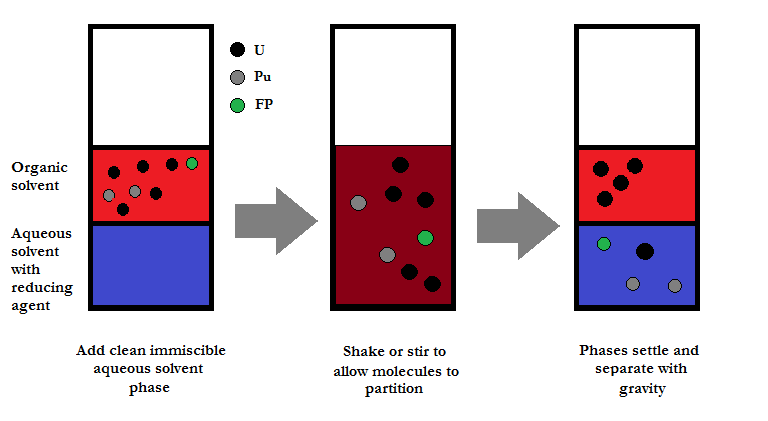
\includegraphics[scale = 0.5]{figures/Back_Extraction}
  %%   \end{center}
  %% \end{figure}
  \begin{figure} \centering
    \vspace*{0.1cm}
    \begin{tikzpicture}[
        every node/.style={anchor=south west,inner sep=0pt},
        x=1mm, y=1mm,
      ]
      \node (fig1) at (0,0)
            {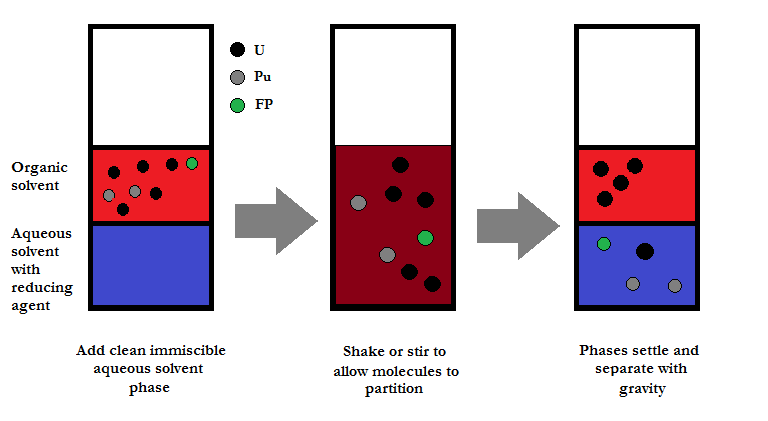
\includegraphics[scale=0.5]{figures/Back_Extraction}};
      \pause
      \node (fig2) at (30,5)
            {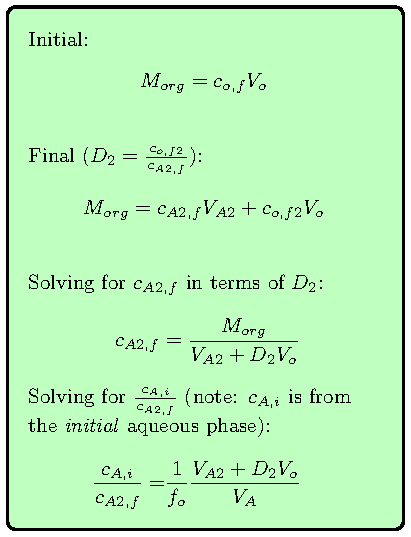
\includegraphics[scale=0.6]{figures/BackExtraction1}};
      \pause
      \node (fig3) at (30,15)
            {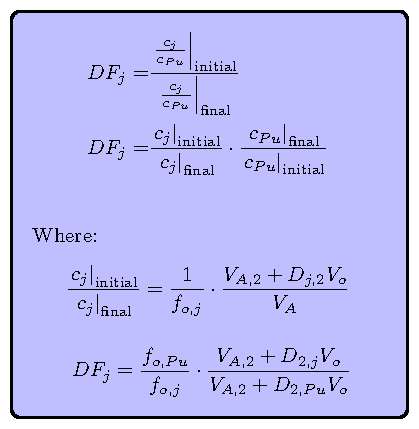
\includegraphics[scale=0.6]{figures/BackExtraction2}};      
            
    \end{tikzpicture}
    \caption{Using Tikz Overlay}
  \end{figure} 
\end{frame}
\note{
  \begin{itemize}
  \item{The fission products that contribute mostly
    to the radioactive contamination of product in PUREX
    are zirconium, niobium, and ruthenium - with multiple
    oxidation states.}
  \end{itemize}
}

%% \begin{frame}{Extraction and Back-extraction}
%%   \begin{columns}
%%     \begin{column}{0.5\textwidth}
%%       \vspace{-3mm}
%%       \begin{itemize}
%%       \item{Extraction}

%%       \item{Back-extraction}
%%         \begin{itemize}
%%           \item{An item}

%%         \end{itemize}
%%       \end{itemize}
%%     \end{column}
%%     \begin{column}{0.5\textwidth}

%%     \end{column}
%%   \end{columns}  
%% \end{frame}


\begin{frame}{Decontamination Factors and their use}
  \begin{itemize}
  \item{After several cycles of Pu extraction/scrubbing/back-extraction
    are completed, the effectiveness of a PUREX cycle is described
    by the decontamination factor (DF):}
    %% \begin{equation*}
    %%   DF_j=\frac{\left|\frac{c_j}{c_{Pu}}\right|_{initial}}
    %%   {\left|\frac{c_j}{c_{Pu}}\right|_{final}}
    %% \end{equation*}
  \item{DFs are characteristic of different process cycles}
  \item{Larger values (10\tss{7}) for industrial scale PUREX (compared
  to benchtop)\tss{\cite{stoller1961reactor,benedict1982nuclear}}}
  \end{itemize}
  \begin{figure}[H]
    \vspace{-3mm}
      \begin{center}
        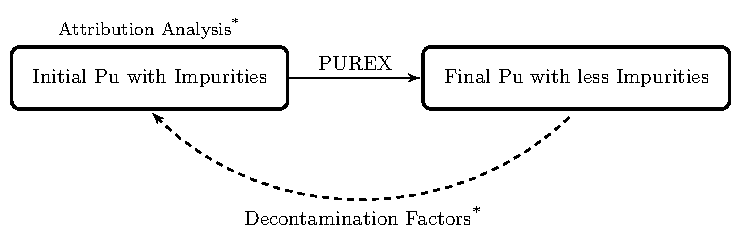
\includegraphics[scale = 0.7]{figures/purpose}
      \end{center}
    \end{figure}
\end{frame}

%% \begin{frame}{Complexity of reprocessing schemes}
%%   \begin{figure}[H]
%%     \vspace*{-1cm}
%%     \begin{center}
%%       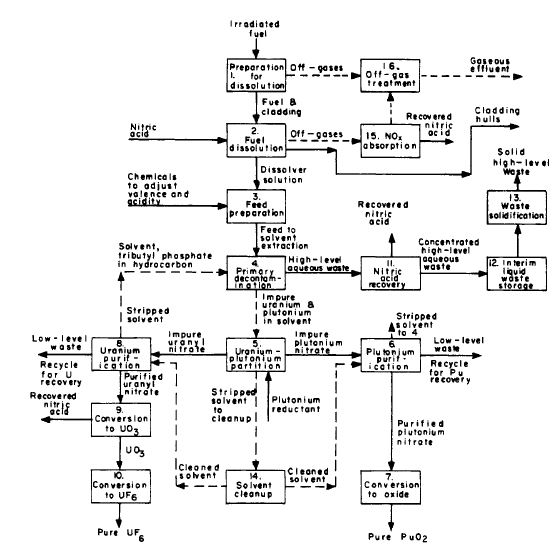
\includegraphics[scale = 0.4]{figures/PUREX_Process}
%%       \caption{\tiny{Principal steps in PUREX\tss{\cite{benedict1982nuclear}}}}
%%     \end{center}
%%   \end{figure}
%%   \note[item]{Worry about dependancies of of DC
%%   Worry about non equilibrium
%%   flow rates, blah blah blah.
%%   Show mixer settler columns, show batch.
%%   What I want to do, get some distribution coefficients
%%   develop a reasonable process for isolating a large
%%   fraction of Pu, then, based on process, calculate what
%%   the decontamination factor should be, and then actually measure it}
%% \end{frame}


%% \begin{frame}{Complexity of reprocessing schemes}
%%   \begin{figure}[H]
%%     \vspace*{-1cm}
%%     \begin{center}
%%       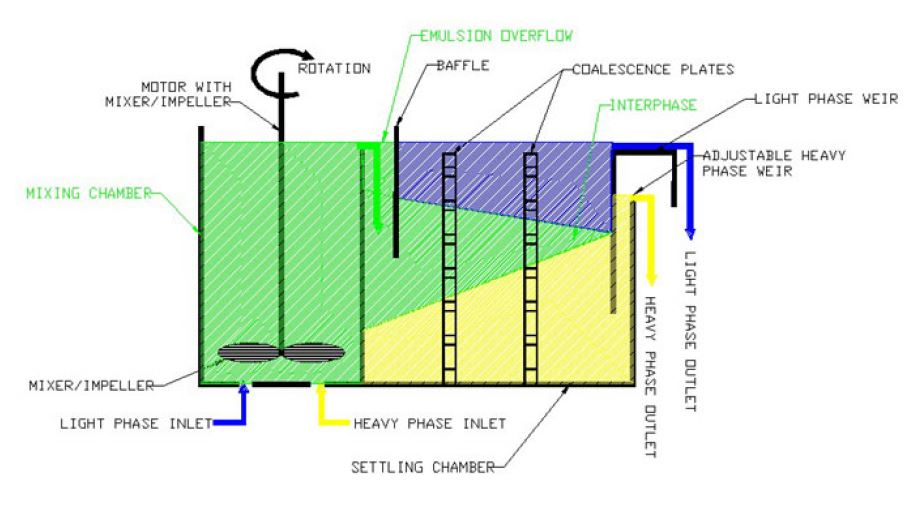
\includegraphics[scale = 0.4]{figures/mixer}
%%       \caption{\tiny{Mixer-Settler Diagram}}
%%     \end{center}
%%   \end{figure}
%% \end{frame}


%% \begin{frame}{Complexity of reprocessing schemes}
%%   \begin{figure}[H]
%%     \vspace*{-1cm}
%%     \begin{center}
%%       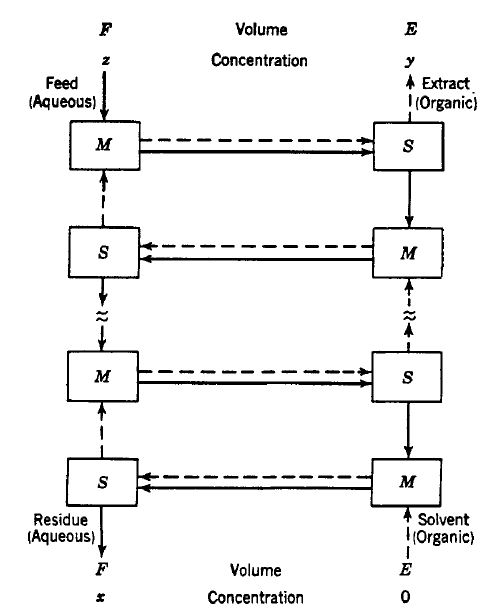
\includegraphics[scale = 0.35]{figures/stage}
%%       \caption{\tiny{Multistage countercurrent solvent extraction.
%%           M, mixer; S, settler.\tss{\cite{benedict1982nuclear}}}}
%%     \end{center}
%%   \end{figure}
%% \end{frame}


%% \begin{frame}{Complexity of reprocessing schemes}
%%   \begin{figure}[H]
%%     \vspace*{-1cm}
%%     \begin{center}
%%       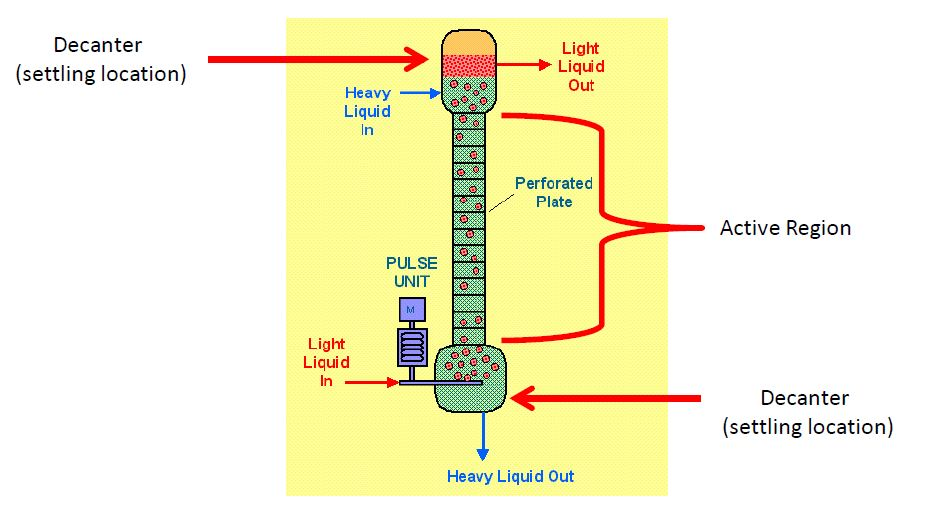
\includegraphics[scale = 0.4]{figures/column}
%%       \caption{\tiny{Pulsed Column Diagram}}
%%     \end{center}
%%   \end{figure}
%% \end{frame}

\section{Objectives}
\begin{frame}[allowframebreaks]{Objectives}
\vspace{-0.7cm}
\textbf{\small Characterize a 4 extraction 3 back-extraction PUREX process}
\begin{itemize}
\item[\notdone]{Collect D-values for each step}
  \begin{itemize}
  \item[\tiny\done]{\tiny \tss{144}Ce,\tss{155}Eu\tss{*},\tss{154}Eu\tss{*},\tss{125}Sb,
    \tss{106}Ru, \tss{134}Cs, \tss{137}Cs
    (Measured Gamma in triplicate)\tss{\cite{chirayath2015trace}}}
  \item[\tiny\done]{\tiny Convert Gamma Spectrum to D-values}
  \item[\tiny\done]{\tiny \tss{85}Rb\tss{*},\tss{90}Sr\tss{*},\tss{97,98,100}Mo,\tss{101,102,104}Ru,
    \tss{110}Pd,\tss{112}Cd,\tss{133}Cs\tss{*},\tss{140,142}Ce,\tss{143}Nd\tss{*},
    \tss{147}Pm\tss{*},\tss{151}Sm\tss{*},\tss{154}Eu\tss{*},U\tss{*},Pu\tss{*} (Mass Spec)}
  \item[\tiny\notdone]{\tiny Convert all mass spec data to D-values}
  \end{itemize}
\item[\notdone]{Collect DF-values for the process}
  \begin{itemize}
  \item[\tiny\done]{\tiny Prepare alpha samples for each step (triplicate)}
  \item[\tiny\notdone]{\tiny Analyze alpha samples for each step}
  \item[\tiny\notdone]{\tiny Convert alpha spec + gamma spec data to DF values}
  \item[\tiny\done]{\tiny Convert Mass spec data to DF values (published)}
  \end{itemize}
\item[\notdone]{Mathematically connect D-values to DFs}
  \begin{itemize}
  \item[\tiny\notdone]{\tiny Derive equations with uncertainty propagation}
  \item[\tiny\notdone]{\tiny Analyze connection with uncertainty}
  \end{itemize}
\end{itemize}
\framebreak
\vspace*{-1cm}
\textbf{\small Determine attribution indicators:}
\begin{itemize}
\item[\notdone]{\small Mathematically derive equations for above indicators with
  respect to one of the isotopes determined above}
  \begin{itemize}
  \item[\tiny\done]{\tiny Burnup}
  \item[\tiny\done]{\tiny Fluence Rate}
  \item[\tiny\done]{\tiny Initial Enrichment}
  \item[\tiny\done]{\tiny Fuel Age}
  \item[\tiny\notdone]{\tiny Fast-to-thermal ratios (requires iteration)}
  \end{itemize}
\item[\notdone]{\small Program a system to iteratively solve for these parameters
  given heavy metal concentration
  ratios}
  \begin{itemize}
  \item[\tiny\notdone]{\tiny Make a program that can read ENDF files for x-sections}
  \item[\tiny\done]{\tiny Create/Use a bateman solver with automated x-section modifications}
  \item[\tiny\done]{\tiny Create program to calculate single group x-sections from
    ENDF data and an assumed
    fast-to-thermal ratio}
  \item[\tiny\notdone]{\tiny Couple all programs together in a single program} 
  \end{itemize}
\item[\notdone]{\small Use above information to determine indicators for three sets of data}
  %% {\tiny
  %% \begin{todolist}
  %% \item{Unprocessed plutonium}
  %% \item{PUREX processed plutonium}
  %% \item{MCNP based reactor modeling and fuel burnup analysis}
  %% \end{todolist}}
\end{itemize}
\end{frame}



\section{Present Status of the Question}
\begin{frame}
\sectionpage
\end{frame}


\begin{frame}
  \begin{itemize}
  \item{Stable noble fission gases as burnup verification\tss{\cite{RN114}}}
  \item{Determine burnup, enrichment, and fuel age from used fuel in a RDD\tss{\cite{RN118}}}
  \item{Analysis of purified plutonium isotopics for reactor type\tss{\cite{RN109}}}
  \item{PUREX co-processing DF values for U and Pu\tss{\cite{RN123}}}
  \item{PUREX D-values and DF values under numerous
    circumstances\tss{\cite{benedict1982nuclear,RN169,RN167,RN168,RN177,stoller1961reactor}}}
    \begin{itemize}
    \item{DF values for \tss{106}Ru and \tss{95}Zr\tss{\cite{stoller1961reactor}}}
    \item{Compilation of D-values for U, Th, and Pu\tss{\cite{RN208}}}
    \item{D-values for rare earths, Pu,
      Th\tss{\cite{RN168,RN181,RN182,RN186,RN179,RN180,RN187,RN185,RN183,RN189}}}
    \item{Ga D-values\tss{\cite{RN189}}}
    \end{itemize}
  \end{itemize}
\end{frame}
\note{
  \begin{enumerate}
  \item{verify burnup so no nefarious activities (we are advancing, because to purified material)
  also Cs is used for burnup}
  \item{RDD not purified, no chemical processing}
  \item{Chem processing, had some difficulty, but some sucess, only looked at differences
    between fast and thermal (not burnup)}
  \item{limited in isotopes solved for}
  \item{Not the isotopes we want}
  \item{Work unique in that elemental DFs used for forensics}
  \end{enumerate}
}



\section{Procedure}
\begin{frame}
  \sectionpage
\end{frame}


%Frame wihout header (if you add the commented out part, the header comes back)
{
  \usebackgroundtemplate{}
  \begin{withoutheadline}
    \begin{frame}%{Analytical Procedure}
      \begin{figure}[H]
        \vspace{-3mm}
        \begin{center}
          \hspace*{-3mm}
          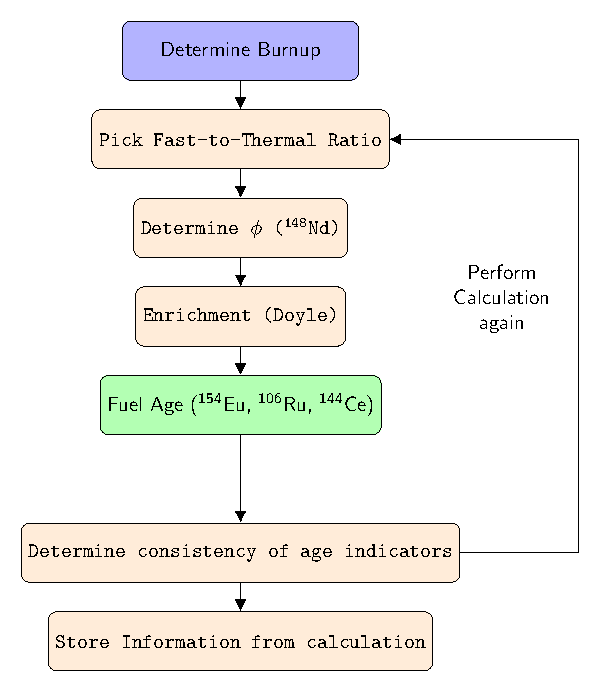
\includegraphics[scale = 0.7]{figures/android.pdf}
        \end{center}
      \end{figure}    
    \end{frame}      
  \end{withoutheadline}
}


\begin{frame}{Analytical Procedure}
  \begin{itemize}
  \item{12.9$\pm$0.1 mg of DUO\tsbs{2} irradiated at HFIR}
  \end{itemize}
  \begin{equation*}
    \frac{dn_i}{dt}=-\lambda_i^{eff}n_i+
    \sum_{j=1}^{N}b_{j\rightarrow i}^{eff}n_j
  \end{equation*}
  \begin{equation*}
    \lambda_i^{eff}=\lambda_i+\phi\sum_{j=1}^N\sigma_{i\rightarrow j}
  \end{equation*}
  \begin{equation*}
    b_{j\rightarrow i}^{eff}=b_{j\rightarrow i}\lambda_j+
      \sigma_{j\rightarrow i}\phi+\gamma_{j\rightarrow i}\sigma_{j,f}\phi
  \end{equation*}
  \begin{equation*}
    \frac{d\vec{n}}{dt}=\bm{A}\vec{n}(t)\rightarrow\vec{n}=e^{\bm{A}t}\vec{n}_0
  \end{equation*}
  %% %The solution to this system is so obvious, I won't even write it down.
  %% \begin{equation*}
  %%   \vec{n}=e^{\bm{A}t}\vec{n}_0
  %% \end{equation*}
\end{frame}
\note{
  Production and loss depend on
  \begin{itemize}
  \item{Neutron Spectra}
  \item{Fluence Rate}
  \item{Cross Section Data}
  \end{itemize}
  Where $N$ is the number of nuclides and blah
  $\gamma_{j\rightarrow i}\ \text{is the fission yield for isotope i from fission of isotope j}$.
  $b_{j\rightarrow i}$ is the fraction of radioactive disintegration by nuclide $j$, which
  leads to nuclide $i$. In the case of spontaneous fission $b_{j\rightarrow i}$ is the product
  of spontenous fission fraction for nuclide $j$ and the yield for fission from nuclide $j$
  producing nuclide $i$.
    Where $\bm{A}$ is a matrix whose diagonal elements are
  $[-\lambda_1^{eff},-\lambda_2^{eff},...,-\lambda_N^{eff}]$,
  all off diagonal elements are
  $b_{j\rightarrow i}^{eff}$ (i for the row, and j is
  for the column) and $\vec{n}(t)=[n_1,n_2,...,n_N]$.
  \textbf{Single Group Cross Section and flux}
}

\begin{frame}{Analytical Procedure - Burnup}
  \begin{align*}    
    BU=&\frac{\text{Power[MW]}\cdot\text{days}}{m[HM]}\\
    =&\left[\frac{N^B}{N_0^{HM}}\right]\frac{N_AE_R}{\gamma_B}\cdot\frac{1}{M_0^{HM}}
  \end{align*}
\end{frame}

\begin{frame}{Analytical Procedure - Fluence Rate}
  \begin{equation*}
    \phi\approx\frac{\lambda_7}{\sigma_7\left(\frac{\gamma_7}{\gamma_8^*-\gamma_8}-1\right)}
  \end{equation*}
\end{frame}

\begin{frame}{Analytical Procedure - Initial Enrichment}
  \begin{align*}
    \epsilon_0=\frac{N^{U238}(T)}{N_0^U}
    \left[\frac{N^{U235}(T)}{N^{U238}(T)}+\frac{N^{U236}(T)}{N^{U238}(T)}\right]+
    \frac{M_0^U}{N_AE_R}BU(T)-G^{238}\\-G^{239}-G^{240}-G^{241}
  \end{align*}
\end{frame}

\begin{frame}{Analytical Procedure - Fuel Age}
  \begin{equation*}
    t_d=-\frac{1}{\lambda}ln\left(\frac{N_\text{measured}}{N_{EOI}}\right)
  \end{equation*}
\end{frame}

\begin{frame}{Analytical Procedure - Fast-to-thermal ratio}
  \begin{itemize}
  \item{Iterative scheme}
  \item{Recalculate the above with new x-sections}
  \item{Cut off for thermal 0.5 ev, 100kev, 20MeV}
  \end{itemize}
\end{frame}


\begin{frame}{Experimental Procedure - Chemistry Procedure}
  \begin{itemize}
  \item{Grab part of procedure from lab notebook, or grab a picture}
  \end{itemize}
\end{frame}

\begin{frame}{Experimental Procedure - Mass Spectrometry}
  
\end{frame}

\begin{frame}{Experimental Procedure - Gamma Spectrometry}

\end{frame}

\begin{frame}{Experimental Procedure - Alpha Spectrometry}

\end{frame}



\section{Current and Expected Results}
\begin{frame}
  \sectionpage
\end{frame}

\subsection{Experiment}
\begin{frame}{Irradiation}
  \begin{columns}
    \begin{column}{0.5\textwidth}
      \vspace{-1cm}
      \begin{itemize}
      \item{12.9 $\pm$ 0.1 mg of DUO\tsbs{2} was irradiated}
        \begin{itemize}
        \item{High Flux Isotope Reactor at Oak Ridge National Laboratory}
        \end{itemize}
      \item{Burnup was 4.43 $\pm$ 0.31 GWd/tHM\tss{\cite{swinney2015experimental}}
       from \tss{137}Cs}
      \item{0.196 $\pm$ mg of total Pu was produced as measured by ICP-MS}
      \end{itemize}
    \end{column}
    \begin{column}{0.5\textwidth}
      \begin{figure}[H]
        \vspace*{-1cm}
        \begin{center}
	   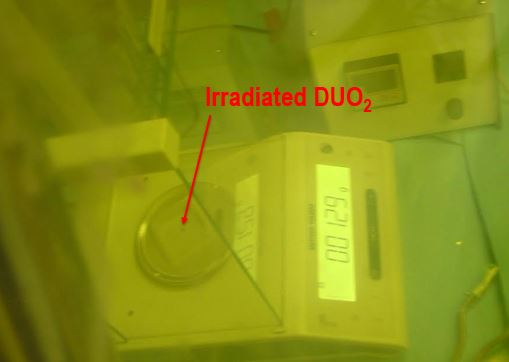
\includegraphics[scale = 0.4]{figures/irradiated}
           %\caption{\tiny{Picture of irradiated sample}}
	\end{center}
      \end{figure}
    \end{column}
  \end{columns}  
  \end{frame}

\begin{frame}{Dissolution of the spent fuel pellet}
      \begin{figure}[H]
        \vspace*{-1cm}
        \begin{center}
	   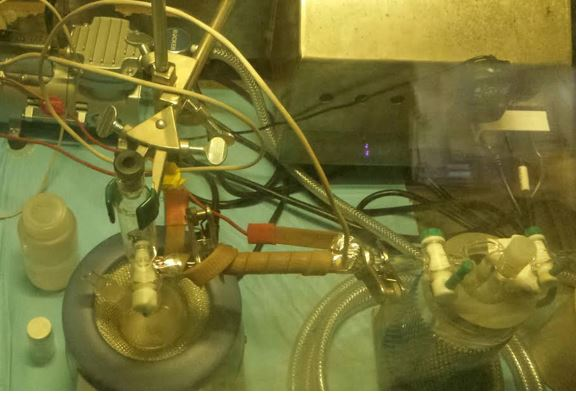
\includegraphics[scale = 0.65]{figures/dissolution}
	\end{center}
      \end{figure}
\end{frame}

\begin{frame}{Glovebox}
      \begin{figure}[H]
        \vspace*{-1cm}
        \begin{center}
	   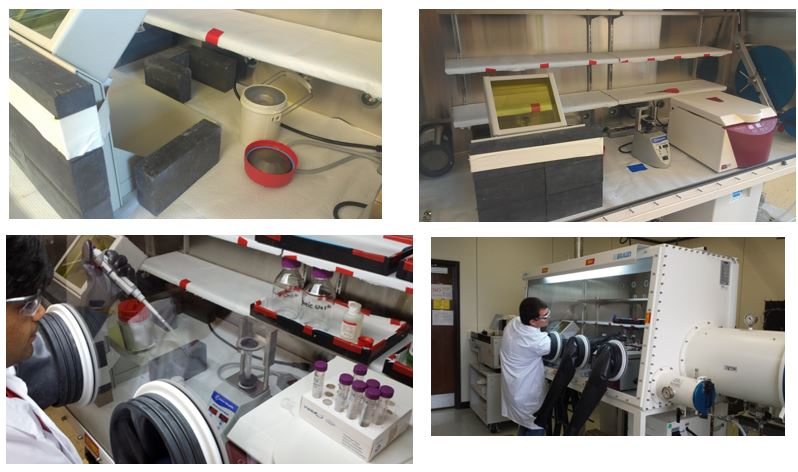
\includegraphics[scale = 0.5]{figures/glovebox}
	\end{center}
      \end{figure}
\end{frame}

\begin{frame}{Experiments}
  \begin{itemize}
  \item{Single stage extraction and back-extraction}
    \begin{itemize}
    \item{Purpose: quantify product recovery, D-values and DF values
      for single stage extraction and back extraction}
    \item{Conditions:}
    \end{itemize}
  \end{itemize}
  \begin{center}
    \vskip -0.2cm
    {\fontsize{2.5}{4}\selectfont
      \begin{tabular}{l  c  c}\toprule
        Starting Solution  & Extraction Solution
        & Back extraction solution \\ \midrule \vspace{0.1cm}
        4 M nitric acid & 30\% vol.\% TBP, 70 vol.\% kerosene & 0.024 M ferrous sulfamate in 0.75 M nitric acid \\ \bottomrule
      \end{tabular}
      }
  \end{center}
  \begin{itemize}
  \item{Multi-contact extraction and back-extraction}
    \begin{itemize}
    \item{Purpose: Quantify DF for a process with 4 extractions,
      3 back extractions}
    \item{Conditions:}
    \end{itemize}
  \end{itemize}
    \begin{center}
    \vskip -0.2cm
    {\fontsize{2.5}{4}\selectfont
      \begin{tabular}{l  c  c}\toprule
        Starting Solution  & Extraction Solution
        & Back extraction solution \\ \midrule \vspace{0.1cm}
        4 M nitric acid & 30\% vol.\% TBP, 70 vol.\% kerosene & 0.024 M ferrous sulfamate in 4 M nitric acid \\ \bottomrule
      \end{tabular}
      }
  \end{center}
\end{frame}

\subsection{Mass Spectrometry}
\begin{frame}{Mass spectrometry Results}
  \begin{block}{Recoveries of U and Pu}
    \begin{center}
      \vskip -0.2cm
   %{\fontsize{2.5}{4}\selectfont
  \begin{tabular}{l  c  c}\toprule
                & Pu Recovery & U Recovery \\ \midrule \vspace{0.1cm}
   Single stage         & (83.4$\pm$9.5)\% & (11.2$\pm$1.3)\% \\
   Multi-contact Cycle 1 & (99.7$\pm$4.2)\% & (6.8$\pm$0.3)\% \\
   Multi-contact Cycle 2 & (93.0$\pm$4.6)\% & (6.6$\pm$0.3)\% \\
   Overall Experiment 2 & (92.7$\pm$6.0)\% & (0.45$\pm$0.03)\% \\ \bottomrule
  \end{tabular}
  %}
  \end{center}
  \end{block}
\end{frame}

\begin{frame}{Mass Spectrometry Results}
  \vspace{-0.6cm}
  \begin{block}{Decontamination Factors}
    \begin{center}
      \vskip -0.2cm
  {\fontsize{7}{11.2}\selectfont
  \begin{tabular}{l  c  c c c c}\toprule
   Element (Z)  & SS & Error & MC Cycle 1 & Error & Isotopes Used\\ \midrule 
   Rb(37) & 39.0 & 5.9 & 11.8 & 0.8 & $^{85}$Rb \\
   Sr(38) & 283  & 43  & 84.6 & 5.9 & $^{90}$Sr \\
   Mo(42) & 5.7  & 0.8 & 1.9  & 0.2 & $^{97,98,100}$Mo \\
   Ru(44) & 59.2 & 6.4 & 16.6 & 2.5 & $^{101,102,104}$Ru \\
   Pd(46) & 65   & 14  & 8.9  & 1.2 & $^{110}$Pd \\
   Cd(48) & 74   & 17  & 22.1 & 2.5 & $^{112}$Cd \\
   Cs(55) & 177  & 28  & 52.9 & 3.9 & $^{133}$Cs \\
   Ce(58) & 43   & 16  & 11.5 & 4.9 & $^{140,142}$Ce \\
   Nd(60) & 19.2 & 2.1 & 5.9  & 0.4 & $^{143}$Nd \\
   Pm(61) & 12.8 & 1.9 & 3.9  & 0.3 & $^{147}$Pm \\
   Sm(62) & 11.5 & 1.5 & 3.6  & 0.3 & $^{151}$Sm \\
   Eu(63) & 10.0 & 1.4 & 3.6  & 0.3 & $^{154}$Eu \\
   U(92) & 7.4   & 1.2 & 14.7 & 0.9 & $^{238}$U \\ \bottomrule
  \end{tabular}
  }
  \end{center}
  \end{block}
\end{frame}


\subsection{Gamma Spectroscopy Results}
\begin{frame}{Gamma Spectroscopy Results}
  %% \vspace{-0.6cm}
  %% \begin{block}{D-Values:}
  %%   \begin{center}
  %%     \vskip -0.2cm
  %% {\fontsize{7}{11.2}\selectfont
  %% \begin{tabular}{l  c  c c c c}\toprule
  %%  Element (Z)  & SS & Error & MC Cycle 1 & Error & Isotopes Used\\ \midrule 
  %%  Rb(37) & 39.0 & 5.9 & 11.8 & 0.8 & $^{85}$Rb \\
  %%  Sr(38) & 283  & 43  & 84.6 & 5.9 & $^{90}$Sr \\
  %%  Mo(42) & 5.7  & 0.8 & 1.9  & 0.2 & $^{97,98,100}$Mo \\
  %%  Ru(44) & 59.2 & 6.4 & 16.6 & 2.5 & $^{101,102,104}$Ru \\
  %%  Pd(46) & 65   & 14  & 8.9  & 1.2 & $^{110}$Pd \\
  %%  Cd(48) & 74   & 17  & 22.1 & 2.5 & $^{112}$Cd \\
  %%  Cs(55) & 177  & 28  & 52.9 & 3.9 & $^{133}$Cs \\
  %%  Ce(58) & 43   & 16  & 11.5 & 4.9 & $^{140,142}$Ce \\
  %%  Nd(60) & 19.2 & 2.1 & 5.9  & 0.4 & $^{143}$Nd \\
  %%  Pm(61) & 12.8 & 1.9 & 3.9  & 0.3 & $^{147}$Pm \\
  %%  Sm(62) & 11.5 & 1.5 & 3.6  & 0.3 & $^{151}$Sm \\
  %%  Eu(63) & 10.0 & 1.4 & 3.6  & 0.3 & $^{154}$Eu \\
  %%  U(92) & 7.4   & 1.2 & 14.7 & 0.9 & $^{238}$U \\ \bottomrule
  %% \end{tabular}
  %% }
  %% \end{center}
  %% \end{block}
\end{frame}

\subsection{Gamma Spectroscopy Results}
\begin{frame}{Initial vs Final solutions}
  \vspace{-0.6cm}
  %% \begin{block}{$c_{A,i}/c_{A,f}$ (Fission Products)}
  %%   \begin{center}
  %%     \vskip -0.2cm
  %% {\fontsize{7}{11.2}\selectfont
  %% \begin{tabular}{l  c  c c c c}\toprule
  %%  Element (Z)  & SS & Error & MC Cycle 1 & Error & Isotopes Used\\ \midrule 
  %%  Rb(37) & 39.0 & 5.9 & 11.8 & 0.8 & $^{85}$Rb \\
  %%  Sr(38) & 283  & 43  & 84.6 & 5.9 & $^{90}$Sr \\
  %%  Mo(42) & 5.7  & 0.8 & 1.9  & 0.2 & $^{97,98,100}$Mo \\
  %%  Ru(44) & 59.2 & 6.4 & 16.6 & 2.5 & $^{101,102,104}$Ru \\
  %%  Pd(46) & 65   & 14  & 8.9  & 1.2 & $^{110}$Pd \\
  %%  Cd(48) & 74   & 17  & 22.1 & 2.5 & $^{112}$Cd \\
  %%  Cs(55) & 177  & 28  & 52.9 & 3.9 & $^{133}$Cs \\
  %%  Ce(58) & 43   & 16  & 11.5 & 4.9 & $^{140,142}$Ce \\
  %%  Nd(60) & 19.2 & 2.1 & 5.9  & 0.4 & $^{143}$Nd \\
  %%  Pm(61) & 12.8 & 1.9 & 3.9  & 0.3 & $^{147}$Pm \\
  %%  Sm(62) & 11.5 & 1.5 & 3.6  & 0.3 & $^{151}$Sm \\
  %%  Eu(63) & 10.0 & 1.4 & 3.6  & 0.3 & $^{154}$Eu \\
  %%  U(92) & 7.4   & 1.2 & 14.7 & 0.9 & $^{238}$U \\ \bottomrule
  %% \end{tabular}
  %% }
  %% \end{center}
  %% \end{block}
\end{frame}

%% \begin{frame}{Conclusions}
%%   \begin{itemize}
%%   \item{Two PUREX experiments were conducted}
%%     \begin{itemize}
%%     \item{Single stage: Determined DC values for Pu, U and several FP}
%%     \item{Multi-contact: Utilized Experiment 1 to recover over 92\%
%%       of Pu while leaving less than 1\% of the U}
%%     \end{itemize}
%%   \item{DF values were measured for 12 FP elements}
%%   \item{DF values were lower than those typically found in industrial
%%     scale PUREX plants due to multiple extraction and back-extraction
%%     steps without an intermittent scrubbing step.}
%%   \item{This work provide DF data that will be built upon for
%%         nuclear forensic investigations of interdicted Pu.}
%%   \end{itemize}
%% \end{frame}

\subsection{Future Work}
\begin{frame}
\subsectionpage
\end{frame}

%% \begin{frame}{Future Work}
%%   \begin{itemize}
%%   \item{Modify Multi-contact extraction, to recover a larger
%%     fraction of Pu}
%%   \item{Investigation of how D-values for (Cs, Sb,
%%     Eu, Rb, Sr, Nd, Pm, and Sm) change as a function of
%%     nitric acid concentration}
%%   \item{Determine statistical uncertainty of D and DF values.}
%%     \begin{itemize}
%%     \item{Repeat above experiments 3-5 times}
%%     \end{itemize}
%%   \item{Connect D-values with process information to DF values}
%% \end{itemize}
%% \end{frame}

\begin{frame}[allowframebreaks]{Objectives}
\vspace{-0.7cm}
\textbf{\small Characterize a 4 extraction 3 back-extraction PUREX process}
\begin{itemize}
\item[\notdone]{Collect D-values for each step}
  \begin{itemize}
  \item[\tiny\done]{\tiny \tss{144}Ce,\tss{155}Eu\tss{*},\tss{154}Eu\tss{*},\tss{125}Sb,
    \tss{106}Ru, \tss{134}Cs, \tss{137}Cs
    (Measured Gamma in triplicate)\tss{\cite{chirayath2015trace}}}
  \item[\tiny\done]{\tiny Convert Gamma Spectrum to D-values}
  \item[\tiny\done]{\tiny \tss{85}Rb\tss{*},\tss{90}Sr\tss{*},\tss{97,98,100}Mo,\tss{101,102,104}Ru,
    \tss{110}Pd,\tss{112}Cd,\tss{133}Cs\tss{*},\tss{140,142}Ce,\tss{143}Nd\tss{*},
    \tss{147}Pm\tss{*},\tss{151}Sm\tss{*},\tss{154}Eu\tss{*},U\tss{*},Pu\tss{*} (Mass Spec)}
  \item[\tiny\notdone]{\tiny Convert all mass spec data to D-values}
  \end{itemize}
\item[\notdone]{Collect DF-values for the process}
  \begin{itemize}
  \item[\tiny\done]{\tiny Prepare alpha samples for each step (triplicate)}
  \item[\tiny\notdone]{\tiny Analyze alpha samples for each step}
  \item[\tiny\notdone]{\tiny Convert alpha spec + gamma spec data to DF values}
  \item[\tiny\done]{\tiny Convert Mass spec data to DF values (published)}
  \end{itemize}
\item[\notdone]{Mathematically connect D-values to DFs}
  \begin{itemize}
  \item[\tiny\notdone]{\tiny Derive equations with uncertainty propagation}
  \item[\tiny\notdone]{\tiny Analyze connection with uncertainty}
  \end{itemize}
\end{itemize}
\framebreak
\vspace*{-1cm}
\textbf{\small Determine attribution indicators:}
\begin{itemize}
\item[\notdone]{\small Mathematically derive equations for above indicators with
  respect to one of the isotopes determined above}
  \begin{itemize}
  \item[\tiny\done]{\tiny Burnup}
  \item[\tiny\done]{\tiny Fluence Rate}
  \item[\tiny\done]{\tiny Initial Enrichment}
  \item[\tiny\done]{\tiny Fuel Age}
  \item[\tiny\notdone]{\tiny Fast-to-thermal ratios (requires iteration)}
  \end{itemize}
\item[\notdone]{\small Program a system to iteratively solve for these parameters
  given heavy metal concentration
  ratios}
  \begin{itemize}
  \item[\tiny\notdone]{\tiny Make a program that can read ENDF files for x-sections}
  \item[\tiny\done]{\tiny Create/Use a bateman solver with automated x-section modifications}
  \item[\tiny\done]{\tiny Create program to calculate single group x-sections from
    ENDF data and an assumed
    fast-to-thermal ratio}
  \item[\tiny\notdone]{\tiny Couple all programs together in a single program} 
  \end{itemize}
\item[\notdone]{\small Use above information to determine indicators for three sets of data}
  %% {\tiny
  %% \begin{todolist}
  %% \item{Unprocessed plutonium}
  %% \item{PUREX processed plutonium}
  %% \item{MCNP based reactor modeling and fuel burnup analysis}
  %% \end{todolist}}
\end{itemize}
\end{frame}




\appendix
\section{Questions?}
\begin{frame}
\sectionpage
\end{frame}

\begin{frame}{Previous Experiment Results}
  \begin{figure}[H]
    \vspace*{-.1cm}
    \begin{center}
      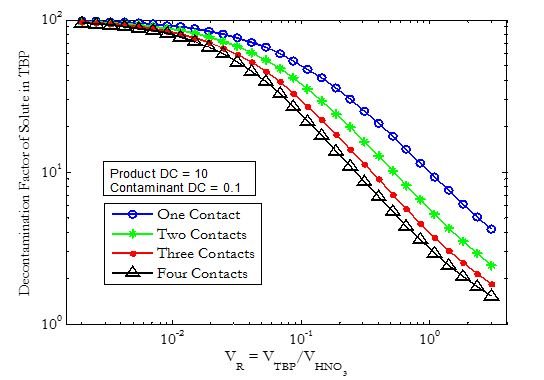
\includegraphics[scale = 0.6]{figures/df}
      \vspace{-0.5cm}
      \caption{\tiny{Decontamination Factors for multi-contact extraction.}}
    \end{center}
  \end{figure}
\end{frame}

\begin{frame}[allowframebreaks]{References}
\def\newblock{}
\nocite{*}
%\scriptsize{\bibliographystyle{plain}}
\scriptsize{\bibliographystyle{unsrt}}
\bibliography{references}
\end{frame}

\begin{frame}{Mass Spec}
  \begin{figure}[H]
    \vspace*{-1cm}
    \begin{center}
      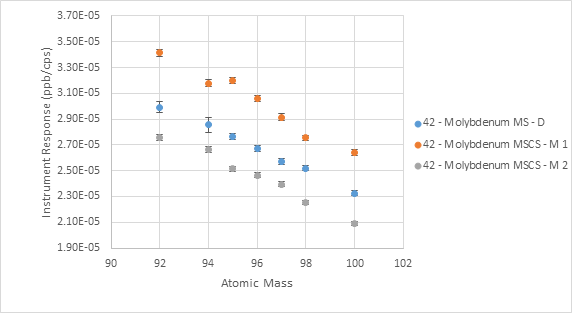
\includegraphics[scale = 0.75]{figures/instrument_response}
    \end{center}
  \end{figure}
\end{frame}

\end{document}
